\section{Extended Evidence and Reproduction Ledger}
\subsection{Acquisition outcome ledger}

The continuation attempted 1 new public YouTube watch request and 1 independent author-transcript request. Successful new operations: 0; new caption documents: 0; new media downloads: 0. The corpus index holds 925 inherited upload metadata records and 0 newly indexed transcript artifacts. The author HTTP 403 and YouTube proxy CONNECT 403 are distinct observations; neither means that a source does not exist.

\subsection{Retained descriptive checks}

Earlier descriptive findings remain available with their original definitions. The caption pilot is shorter in median duration than the nonpilot known-duration pool; title-keyword duration contrasts change with per-account weighting; the former 22-video/eleven-account centroid comparison is distinct from the new 25-video upload-pair diagnostic. They provide context rather than independent replication of the continuation analyses.

\begin{figure*}[t]
\centering
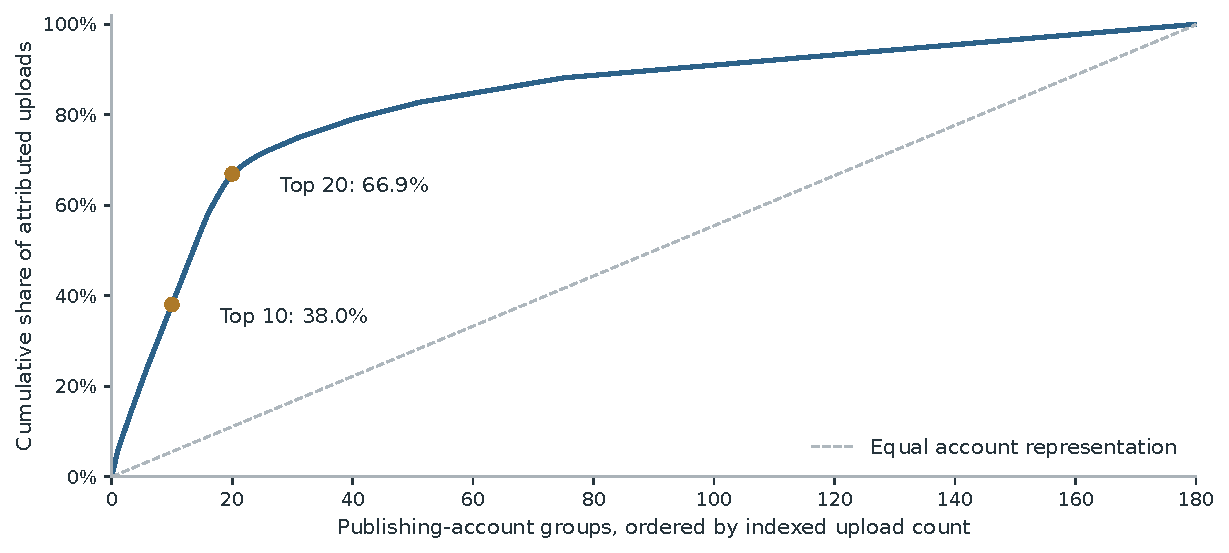
\includegraphics[width=\textwidth]{generated/figures/retained-concentration.pdf}
\caption{Retained publisher concentration among attributed indexed uploads, not population prevalence.}
\label{fig:retained-concentration}
\end{figure*}

\begin{figure*}[t]
\centering
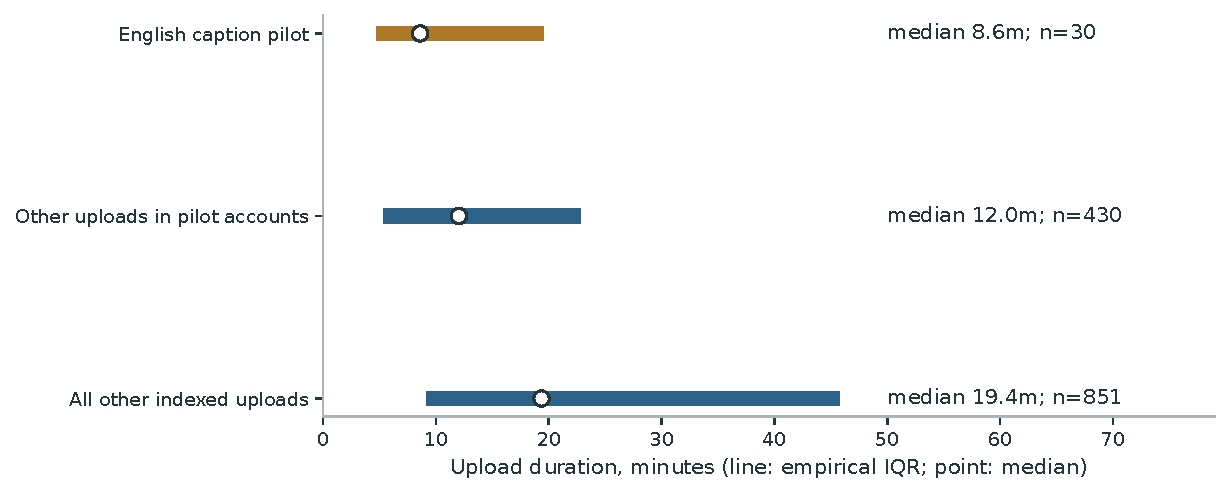
\includegraphics[width=\textwidth]{generated/figures/retained-caption-selection.pdf}
\caption{Retained selected-caption duration comparison. Interquartile spans are empirical distributions, not confidence intervals.}
\label{fig:retained-caption-selection}
\end{figure*}

\begin{figure*}[t]
\centering
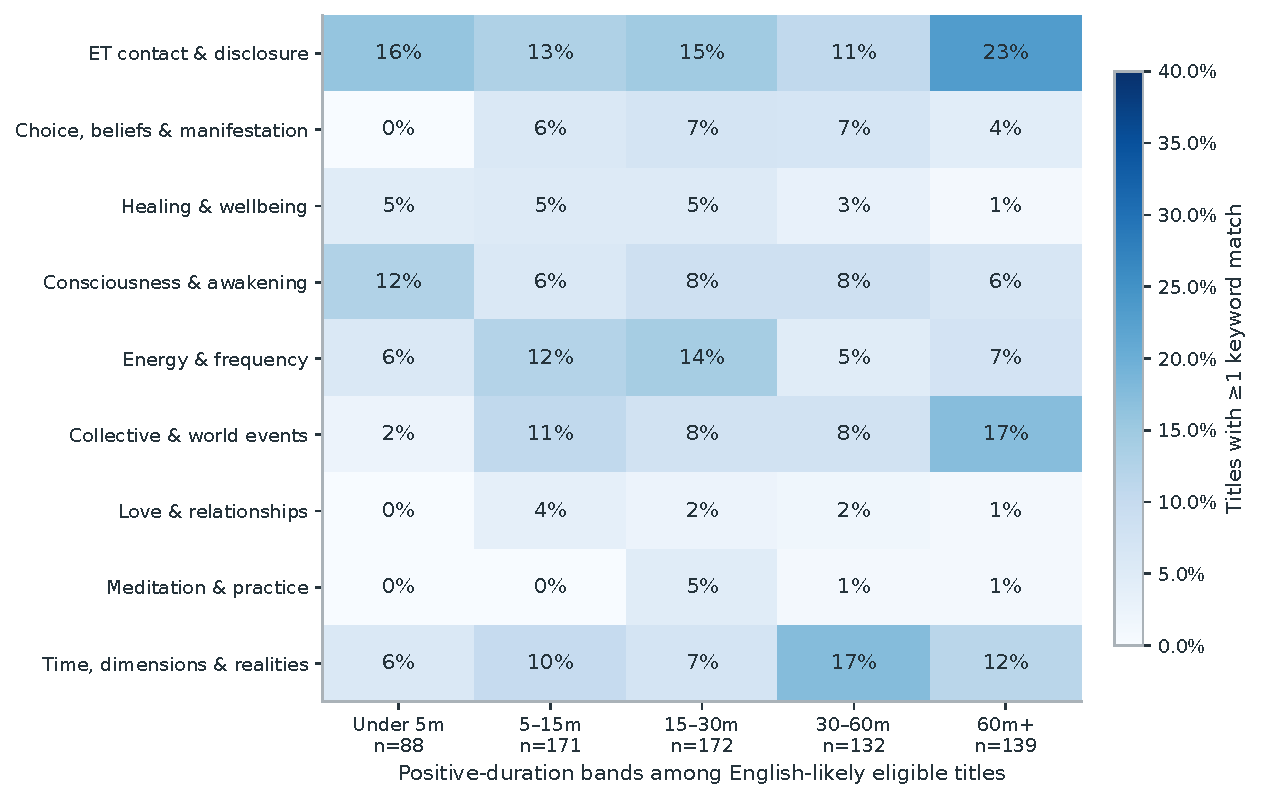
\includegraphics[width=\textwidth]{generated/figures/retained-keyword-duration.pdf}
\caption{Retained title keyword presence by measured duration. The 702 eligible titled uploads with known duration define the denominator; overlapping dictionary families are unvalidated indicators.}
\label{fig:retained-keyword-duration}
\end{figure*}

\subsection{Lexical source-family rule sensitivity}

The stricter proxy requires repeated question-pair links at each listed cosine threshold. Its group counts describe that alternative rule, rather than the more inclusive guard used to split the local-model pilot. Neither rule verifies original-session identity.

\begin{table}[t]
\centering\small\setlength{\tabcolsep}{3pt}
\begin{tabular}{p{0.23\columnwidth}p{0.23\columnwidth}p{0.23\columnwidth}p{0.2\columnwidth}}
\toprule
Min cosine & Links needed & Upload links & Groups \\ \midrule
0.70 & 2 & 6 & 62 \\
0.80 & 2 & 4 & 64 \\
0.90 & 2 & 4 & 64 \\
\bottomrule
\end{tabular}
\caption{Stricter repeated-question-pair source proxy. This rule differs from the more inclusive benchmark guard and must not be described as the same session classification.}
\end{table}

\subsection{Model-assisted reading artifacts}

The retained repository files \path{research/expansion/qa/close-reading.json} and \path{research/expansion/qa/pair-close-reading.json} contain twenty single-candidate and twelve paired model-assisted readings, respectively. Each links to digest source pointers and hashes. The inspected material is the existing AI-generated question and gist fields; no human annotation, raw transcript, audio or video inspection is claimed by these ledgers. All paired answer-agreement fields remain undetermined.

One paired reading identifies compatible life-purpose paraphrases despite different answer wording; another retains uncertainty about relative versus calendar contact windows because original recording dates are unresolved. These interpretations illustrate why a lexical score alone cannot establish contradiction or chronological drift. They are selected interpretive examples, not a representative validation sample.


\section{Evidence Types and Interpretation}
A watch-page response supports observed metadata at retrieval. A title supports publishing-language analysis. An offered caption supports analysis of its available text and flags, with recognition and speaker limitations. A digest Q\&A row supports source-linked paraphrase retrieval. A frozen embedding supports numerical comparisons on its original items. A generated answer supports inspection of that model's behavior under its prompt and accessible evidence. These are distinct observations.

We separate four practical questions: does a statement resemble another text; does it accurately reproduce a source account; does a source support the asserted proposition; and is that proposition externally verified? The current automatic measures mainly address the first, with source-ID checks contributing limited evidence about the second and third. They do not settle external verification.

\section{Dataset and Model Update Procedure}
Preserve raw-source provenance, source access depth and earlier releases. Define the unit and inclusion rules before expanding collection. Execute a small access pilot, retain failures and success hashes, and distinguish new retrieval from reuse of frozen derivatives. When new source text becomes available, record its permission/release basis, caption type, language, timestamps and speaker uncertainty.

Regenerate relevant statistics, keyword features, source families, splits and model runs when inputs change. Repin models by immutable revision and verified artifact hash. Keep source/video grouping and retrieval evidence fixed across comparable arms; separately report any deliberate change in context budget or adaptation data. Review affected prose and figures rather than allowing automatically updated counts to coexist with stale interpretations.

The paper build uses deterministic metadata, current generated values, fixed figure files and the unchanged official style. The standalone source ZIP compiles the manuscript; the repository experiment scripts reconstruct the analytical outputs. Byte-identical same-environment rebuilding and clean-package page-text checks are separate capabilities. Full model recomputation also requires the pinned model artifacts and runtime, which are not silently bundled as manuscript text.

\section{Future Studies and Falsifiers}
\paragraph{Matched answers across practitioners.} Obtain equivalent prompts and complete attributable answers from more than one practitioner, group original performances and code agreement, qualification, disagreement and indeterminate separately from topic. The hypothesis that high lexical neighbors are equivalent prompts fails if blinded judgments mostly identify materially different or underspecified questions. A useful plot is a prompt-by-practitioner answer-relation matrix with missing cells and source counts.

\paragraph{Speaker and context windows.} Human-check host, question, message and promotion intervals, then compare whole recordings with the same items' attributed-message windows. Improved substantive retrieval is disconfirmed if held-out relevance does not improve. Plot paired neighbor changes with exclusions; do not describe positional trimming as diarization.

\paragraph{Original-session reuse.} Confirm edit/repost families with explicit source links and authorized audiovisual evidence, then collapse to one performance unit. An apparent independent cross-account relation weakens if it disappears on collapse. A bipartite upload/session graph can reveal this dependence without asserting direction from similarity alone.

\paragraph{Chronological change.} Obtain original recording dates and sufficiently complete histories, then test within-source changes with format and reuse controlled. A drift hypothesis fails when it vanishes under these controls. Time plots should show denominators, missing intervals and the meaning of uncertainty.

\paragraph{Human validation of retrieval and generation.} Use blinded, held-out prompt-equivalence, source-entailment and answer-relation judgments, with a documented codebook and adjudication. Model improvement fails if it does not exceed an equal-evidence lexical baseline on those judgments. Token-overlap gains alone do not satisfy the criterion.

\paragraph{Multilingual and caption accuracy.} Compare licensed pinned encoders on identical human-reviewed language strata, and audit speech recognition against corrected reference segments. Record word/claim error, speaker confusion and missed questions. A model or caption threshold fails if held-out errors exceed the predefined standard or change extracted claims.

\paragraph{Uncertainty and conditionality.} Annotate propositions, negation, quoted speech, time windows and conditions from original answer spans. Test lexical marker retrieval against held-out labels rather than equating marker counts with certainty, sincerity or deception. Confusion matrices and within-prompt distributions should retain indeterminate cases.

These are unexecuted research directions unless a separate dated result artifact explicitly reports their execution. No future-study row is an empirical finding.

\section{Pending Human and Submission Decisions}
Human authorship and affiliations; contributor review and factual acceptance; institutional ethics determination for the actual study design; release-rights review; human construct and caption validation; a concrete venue; current checklist answers; disclosure placement; and submission approval remain TBD. The ICWSM 2027 initial-paper guidance checked for this phase states eleven pages including references, with checklist and appendices separate. This living manuscript prioritizes inspectability and does not claim automatic compliance with that limit or final checklist.
